\section{Auswertung}
Mit dem Aufbau ist es möglich Geschwindigkeiten bis zu 200 $\nicefrac{km}{h}$ zu generieren. Wie \ref{fig:AuswertungSpeed} zeigt, nimmt der Fehler zu, je höher die Geschwindigkeit ist. Dieses Verhalten zeigt auch \ref{fig:AuswertungZeitfehler}. Der gemessene \marg{Fehler} Fehler liegt jedoch unter 6\%.\\
\begin{figure}[ht]
    \centering
    %    \missingfigure{Bild einfügen}
    \includegraphics[width=\textwidth]{images/auswertungSpeedUeb.png}
    \caption{Vergleich unterschiedliche Geschwindigkeiten}
    \label{fig:AuswertungSpeed}
\end{figure}

In \ref{fig:AuswertungInt} \marg{Vergleich Polling - Interrupt} werden die verschiedene Implementationsmethoden verglichen.
Die Daten für Puls LS1 und Puls LS2 wurden durch Polling gewonnen während die restlichen durch Interrupts generiert wurden. Detailliertere Grafiken dazu finden sich in Anhang \ref{app:Auswertung}.
\begin{figure}[ht]
    \centering
%    \missingfigure{Bild einfügen}
    	\includegraphics[width=\textwidth]{images/auswertungInt.png}
    \caption{Vergleich Interrupt und Polling bei 1000 RPM (94.2 $\nicefrac{km}{h}$)}
    \label{fig:AuswertungInt}
\end{figure}

\clearpage
\subsection{Fehlerquellen}
Die \ref{fig:AuswertungZeitfehler} zeigt den maximalen Geschwindigkeitsfehler wenn mit der maximalen Ansprechzeit der Lichtschranke von 0.5ms gerechnet wird.
\begin{figure}[ht]
    \centering
    %    \missingfigure{Bild einfügen}
    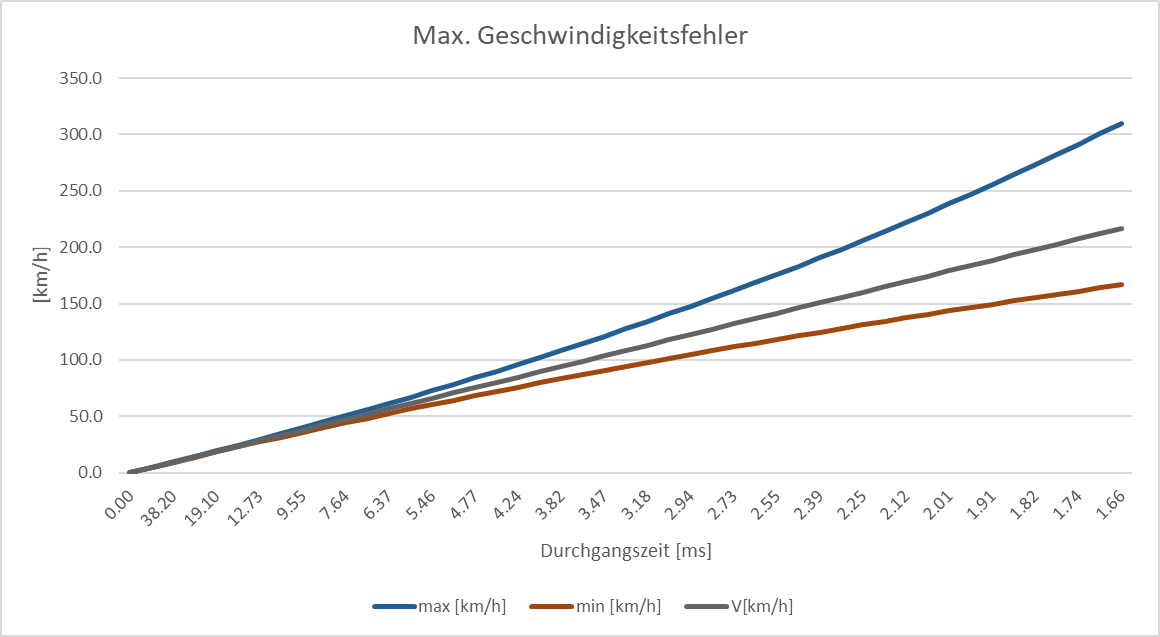
\includegraphics[width=\textwidth]{images/Zeitfehler.png}
    \caption{Max. Geschwindigkeitsfehler maximaler Ansprechverzögerung.}
    \label{fig:AuswertungZeitfehler}
\end{figure}

Die für diesen Versuchsaufbau relevanten \marg{Fehlerquellen}Fehlerquellen sind:
\begin{itemize}
    \item Ungenauer Abstand der Lichtschranken zueinander.
    \item Ungenauer Abstand der Lichtschranken zum Drehpunkt des Rotors.
    \item Ungenauigkeit infolge der Reaktionszeit der Lichtschranke.
    \item Ungenauigkeit infolge Regelabweichung des Motors.
    \item Ungenauigkeit infolge der Reaktionszeit des Arduinos.
\end{itemize}
